% =====================================================================
%  Carga dinámica: balanceo estático vs dinámico (Maestro-Trabajador)
%  Compilar:  pdflatex main.tex   (2 veces)   [18 diapositivas; el código va aparte]
%  Guion del expositor:  python guion.py && pdflatex guion.tex
%  Antes: python ../tabla_latex.py   (genera numeros.tex y tabla_resumen.tex)
% =====================================================================
\documentclass[aspectratio=169,11pt,t]{beamer}

\usepackage[utf8]{inputenc}
\usepackage[T1]{fontenc}
\usepackage{lmodern}
\IfFileExists{spanish.ldf}{\usepackage[spanish,es-noshorthands]{babel}}{\usepackage[english]{babel}}
\usepackage{microtype}
\usepackage{booktabs,array,colortbl,graphicx,amsmath,listings}
\usepackage{tikz}
\usetikzlibrary{arrows.meta,positioning,shapes.geometric,fit,calc,patterns,decorations.pathreplacing,backgrounds}
\usepackage[most]{tcolorbox}
\tcbuselibrary{skins}

% ---------- datos de la portada (cámbialos aquí) ----------
\newcommand{\materia}{Cómputo Paralelo Distribuido}
\newcommand{\integrantes}{Jared Méndez Valencia\\Daniel del Valle Andrade\\Johan Lezama Núñez\\Camila Serrano Trinidad}
\newcommand{\grupo}{7C}
\newcommand{\carrera}{Ingeniería en Sistemas y Tecnología de la Información}

% Generado por tabla_latex.py - no editar a mano
\newcommand{\tEstHet}{2.41}
\newcommand{\tCicHet}{2.29}
\newcommand{\tPondHet}{0.91}
\newcommand{\tDinUnoHet}{0.84}
\newcommand{\tDinHet}{0.92}
\newcommand{\tGuiHet}{1.05}
\newcommand{\tEstHom}{0.63}
\newcommand{\tDinHom}{0.62}
\newcommand{\tIdealHet}{0.80}
\newcommand{\tUnNodoHet}{2.21}
\newcommand{\tEstDeg}{1.53}
\newcommand{\tCicDeg}{1.24}
\newcommand{\tDinDeg}{0.75}
\newcommand{\tGuiDeg}{0.65}
\newcommand{\spEstHet}{0.92}
\newcommand{\spDinHet}{2.39}
\newcommand{\efDinHet}{87}
\newcommand{\efEstHet}{33}
\newcommand{\utEstHet}{49}
\newcommand{\utDinHet}{91}
\newcommand{\mejoraHet}{2.6}
\newcommand{\mejoraDeg}{2.0}
\newcommand{\chunkMejor}{2}
\newcommand{\tChunkMejor}{0.97}
\newcommand{\chunkPeor}{60}
\newcommand{\tChunkPeor}{2.43}
\newcommand{\spDinOcho}{4.9}
\newcommand{\spEstOcho}{1.9}


% ---------- paleta: "consola de control" ----------
\definecolor{fondo}{HTML}{1A1A19}
\definecolor{panel}{HTML}{262624}
\definecolor{tinta}{HTML}{F0EFEC}
\definecolor{tinta2}{HTML}{C3C2B7}
\definecolor{azul}{HTML}{3987E5}
\definecolor{naranja}{HTML}{D95926}
\definecolor{aqua}{HTML}{199E70}
\definecolor{ambar}{HTML}{C98500}
\definecolor{rosa}{HTML}{D55181}

\setbeamercolor{background canvas}{bg=fondo}
\setbeamercolor{normal text}{fg=tinta}
\setbeamercolor{structure}{fg=azul}
\setbeamercolor{frametitle}{fg=tinta}
\setbeamercolor{footline}{fg=tinta2,bg=fondo}
\setbeamercolor{note page}{bg=white,fg=black}
\setbeamercolor{note title}{bg=white,fg=black}
\setbeamerfont{frametitle}{size=\Large,series=\bfseries}
\renewcommand{\familydefault}{\sfdefault}
\setbeamertemplate{navigation symbols}{}
\setbeamersize{text margin left=1.1cm,text margin right=1.1cm}
\setbeamertemplate{itemize item}{\color{azul}\tiny$\blacksquare$}
\setbeamertemplate{itemize subitem}{\color{naranja}\tiny$\blacksquare$}
\setbeamerfont{itemize/enumerate body}{size=\normalsize}
\setlength{\leftmargini}{1.1em}

\setbeamertemplate{frametitle}{%
  \nointerlineskip\vskip 0.9ex
  {\fontsize{7}{8}\selectfont\ttfamily\color{azul}\MakeUppercase{\insertsection}}\par
  \vskip 0.2ex
  {\usebeamerfont{frametitle}\usebeamercolor[fg]{frametitle}\insertframetitle\par}
  \vskip 0.4ex
  {\color{naranja}\rule{1.2cm}{2.4pt}}\par\vskip -0.3cm}

\setbeamertemplate{footline}{%
  \leavevmode
  \begin{tikzpicture}[remember picture,overlay]
    \pgfmathsetmacro{\fraccionprog}{\insertframenumber/\inserttotalframenumber}
    \pgfmathsetlengthmacro{\anchoprog}{\fraccionprog*\paperwidth}
    \fill[panel] (current page.south west) rectangle ++(\paperwidth,2pt);
    \fill[azul] (current page.south west) rectangle ++(\anchoprog,2pt);
  \end{tikzpicture}%
  \hbox to \paperwidth{\hspace*{1.1cm}%
    {\fontsize{6.5}{8}\selectfont\ttfamily\color{tinta2}UVP · \materia\hfill
     \insertframenumber\,/\,\inserttotalframenumber}\hspace*{1.1cm}}%
  \vskip 1.1ex}

% ---------- tarjetas ----------
\newtcolorbox{tarjeta}[3][]{enhanced,colback=panel,colframe=panel,boxrule=0pt,arc=3pt,
  borderline west={3pt}{0pt}{#2},left=9pt,right=6pt,top=5pt,bottom=5pt,
  before upper={{\bfseries\color{#2}#3}\par\vspace{2pt}},fontupper=\small\raggedright\color{tinta},#1}
\newcommand{\ok}[1]{\leavevmode{\color{aqua}#1}}
\newcommand{\ko}[1]{\leavevmode{\color{naranja}#1}}
\newcommand{\mono}[1]{\leavevmode{\ttfamily\color{ambar}#1}}
\newcommand{\fuente}[1]{\vfill{\fontsize{7}{8}\selectfont\color{tinta2}#1}}
\renewcommand{\arraystretch}{1.25}

% ---------- estilos de TikZ ----------
\tikzset{
  nodo/.style={rounded corners=3pt,fill=panel,draw=tinta2!45,line width=.6pt,
    inner sep=4pt,text=tinta,font=\small,align=center},
  flecha/.style={-{Stealth[length=5pt]},line width=.9pt,color=tinta2},
  txtp/.style={font=\scriptsize,text=tinta2},
  txtm/.style={font=\ttfamily\scriptsize,text=ambar},
}

% ---------- código ----------
\lstdefinelanguage{pseudo}{morekeywords={PARA,CADA,EN,MIENTRAS,SI,ENTONCES,SINO,
  REPETIR,ENVIAR,RECIBIR,SCATTER,BARRERA,salir,hasta},sensitive=true,
  morecomment=[l]{//}}
\lstset{
  basicstyle=\ttfamily\fontsize{7}{8.4}\selectfont\color{tinta},
  keywordstyle=\color{azul}\bfseries,commentstyle=\color{aqua}\itshape,
  stringstyle=\color{ambar},numberstyle=\tiny\color{tinta2},
  backgroundcolor=\color{panel},frame=single,rulecolor=\color{panel},framesep=5pt,
  xleftmargin=5pt,xrightmargin=0pt,showstringspaces=false,breaklines=true,
  keepspaces=true,columns=fullflexible,aboveskip=2pt,belowskip=0pt,
  literate={á}{{\'a}}1 {é}{{\'e}}1 {í}{{\'i}}1 {ó}{{\'o}}1 {ú}{{\'u}}1
           {Á}{{\'A}}1 {É}{{\'E}}1 {Í}{{\'I}}1 {Ó}{{\'O}}1 {Ú}{{\'U}}1
           {ñ}{{\~n}}1 {Ñ}{{\~N}}1 {¿}{{?`}}1 {¡}{{!`}}1 {ü}{{\"u}}1
           {<-}{{$\leftarrow$}}1 {->}{{$\rightarrow$}}1,
}
\lstdefinestyle{py}{language=Python,numbers=left,numbersep=6pt,basicstyle=\ttfamily\fontsize{6.8}{8}\selectfont\color{tinta}}
\lstdefinestyle{ps}{language=pseudo}
\lstdefinestyle{term}{language={},basicstyle=\ttfamily\fontsize{6.8}{8.2}\selectfont\color{tinta2}}

\begin{document}

\begin{frame}[plain]
\begin{tikzpicture}[remember picture,overlay]
  % motivo: línea de tiempo estático (hachurado) vs dinámico
  \begin{scope}[shift={($(current page.north east)+(-5.9,-2.6)$)}]
    \foreach \i/\d in {0/1.2,1/1.2,2/2.4,3/4.8}{
      \fill[naranja] (0,{-\i*.55}) rectangle (\d,{-\i*.55-.34});
      \fill[pattern=north east lines,pattern color=tinta2!60] (\d,{-\i*.55}) rectangle (4.8,{-\i*.55-.34});
    }
    \foreach \i/\n/\w in {0/5/.96,1/5/.96,2/2.5/1.92,3/1/4.8}{
      \foreach \k in {1,...,5}{
        \ifnum\k>\n\relax\else
        \pgfmathsetmacro{\xa}{(\k-1)*\w}
        \pgfmathsetmacro{\xb}{\k*\w-.05}
        \fill[azul] ({\xa},{-\i*.55-2.8}) rectangle ({\xb},{-\i*.55-2.8-.34});
        \fi}
    }
    \node[txtm,anchor=west] at (0,.35) {estático};
    \node[txtm,anchor=west] at (0,-2.45) {dinámico};
  \end{scope}
  \fill[naranja] ($(current page.north west)+(1.1,-2.1)$) rectangle ++(.09,3.3);
\end{tikzpicture}
\vspace*{.6cm}
\hspace*{.35cm}\begin{minipage}{.56\textwidth}
  {\fontsize{7.5}{9}\selectfont\ttfamily\color{azul}EXPOSICIÓN · TEMA}\\[2pt]
  {\fontsize{30}{32}\selectfont\bfseries\color{tinta}Carga dinámica}\\[5pt]
  {\large\color{tinta2}Balanceo de carga estático vs.\ dinámico en una arquitectura Maestro–Trabajador}\\[.45cm]
  {\color{tinta}\bfseries Alumnos:}\\[1pt]
  {\small\color{tinta}\integrantes}\\[4pt]
  {\small\color{tinta2}\carrera}\\[1pt]
  {\small\color{tinta2}UVP · \materia · Grupo \grupo}
\end{minipage}
\note[item]{Presentación del equipo: cada integrante dice su nombre y qué parte expone.}
\note[item]{Frase gancho: ``¿Qué pasa cuando un nodo lento frena a uno rápido?'' Hoy lo vemos con teoría y con una simulación en una laptop.}
\end{frame}

\section{Introducción}
\begin{frame}{Objetivos}
\begin{tarjeta}[]{azul}{Objetivo general}\small 
Comprender y comparar el balanceo de carga \textbf{estático} y \textbf{dinámico} en una arquitectura
\textbf{Maestro–Trabajador}, y demostrarlo con una simulación en MPI.
\end{tarjeta}\vspace{2pt}
\begin{columns}[T,onlytextwidth]
\column{.49\textwidth}
\begin{tarjeta}[height=1.3cm]{naranja}{1 · Explicar}
Cómo se reparte el trabajo para que un nodo lento \textbf{no frene} a uno rápido.
\end{tarjeta}\vspace{4pt}
\begin{tarjeta}[height=1.3cm]{aqua}{3 · Proponer}
Estrategias para \textbf{evitar nodos en espera}.
\end{tarjeta}
\column{.49\textwidth}
\begin{tarjeta}[height=1.3cm]{azul}{2 · Comparar}
El algoritmo estático vs.\ el dinámico (paquetes según la velocidad de los nodos).
\end{tarjeta}\vspace{4pt}
\begin{tarjeta}[height=1.3cm]{ambar}{4 · Medir}
Tiempo, speedup, eficiencia y ocio con código en Python + mpi4py.
\end{tarjeta}
\end{columns}
\note[item]{Los cuatro objetivos específicos coinciden con lo que pide el tema: cómo se reparte, algoritmo estático vs dinámico, paquetes según velocidad y estrategias para evitar nodos en espera.}
\end{frame}

\section{El problema}
\begin{frame}{Un nodo lento frena a uno rápido}
\centering
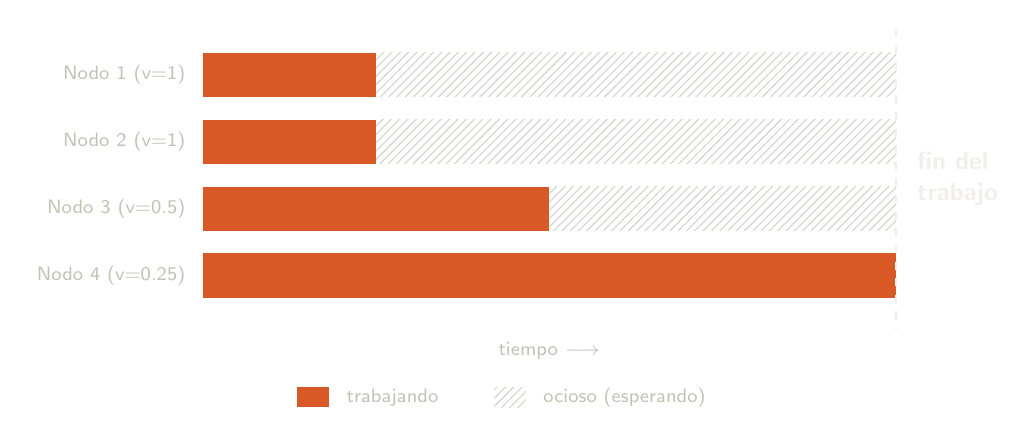
\begin{tikzpicture}
  \foreach \i/\d/\n in {0/2.2/{Nodo 1  (v=1)},1/2.2/{Nodo 2  (v=1)},2/4.4/{Nodo 3  (v=0.5)},3/8.8/{Nodo 4  (v=0.25)}}{
    \node[txtp,anchor=east] at (-.1,{-\i*.85-.28}) {\n};
    \fill[naranja] (0,{-\i*.85}) rectangle ({\d},{-\i*.85-.56});
    \fill[pattern=north east lines,pattern color=tinta2!70] ({\d},{-\i*.85}) rectangle (8.8,{-\i*.85-.56});
  }
  \draw[dashed,tinta,line width=1pt] (8.8,.3) -- (8.8,-3.5);
  \node[font=\small\bfseries,text=tinta,anchor=west,align=left] at (8.95,-1.6) {fin del\\trabajo};
  \node[txtp,anchor=north] at (4.4,-3.55) {tiempo $\longrightarrow$};
  \fill[naranja] (1.2,-4.5) rectangle ++(.4,.25); \node[txtp,anchor=west] at (1.7,-4.38) {trabajando};
  \fill[pattern=north east lines,pattern color=tinta2!70] (3.7,-4.5) rectangle ++(.4,.25);
  \node[txtp,anchor=west] at (4.2,-4.38) {ocioso (esperando)};
\end{tikzpicture}\\[6pt]
{\large Reparto igual para todos $\Rightarrow$ $T_{\text{total}}=\max_i T_i$ y los rápidos \ko{esperan}}
\note[item]{Aquí está la idea central de todo el tema: con un reparto igual, el trabajo termina cuando termina el nodo más lento.}
\note[item]{Los nodos rápidos quedan ociosos: se paga hardware que no se aprovecha.}
\end{frame}

\begin{frame}{Conceptos y métricas}
\begin{columns}[T,onlytextwidth]
\column{.44\textwidth}
\begin{tarjeta}[]{azul}{Conceptos clave}
\begin{itemize}\setlength\itemsep{2pt}\footnotesize
\item \textbf{Nodo}: procesador o máquina (aquí, un proceso MPI)
\item \textbf{Tarea}: unidad de trabajo con un costo
\item \textbf{Paquete (chunk)}: tareas que se entregan juntas
\item \textbf{Maestro}: reparte y coordina, no calcula
\item \textbf{Trabajador}: ejecuta paquetes y pide más
\item \textbf{Heterogeneidad}: velocidades $v_i$ distintas
\end{itemize}
\end{tarjeta}
\column{.54\textwidth}
\begin{tarjeta}[height=.95cm]{naranja}{Tiempo total (makespan)}
\small $T=\max_i T_i$
\end{tarjeta}\vspace{1pt}
\begin{tarjeta}[height=.95cm]{aqua}{Speedup}
\small $S=T_{\text{1 nodo rápido}}\,/\,T_{\text{real}}$
\end{tarjeta}\vspace{1pt}
\begin{tarjeta}[height=.95cm]{azul}{Eficiencia de balanceo}
\small $E=T_{\text{ideal}}/T_{\text{real}}$,\quad $T_{\text{ideal}}=\sum c_j/\sum v_i$
\end{tarjeta}\vspace{1pt}
\begin{tarjeta}[height=.95cm]{ambar}{Utilización}
\small $U=\text{ocupado}/T$,\quad ocio $=T-\text{ocupado}$
\end{tarjeta}
\end{columns}
\note[item]{Define con tus palabras cada concepto; son el vocabulario del resto de la exposición.}
\note[item]{El ideal es el balance perfecto sin costos de comunicación: el trabajo total entre la suma de velocidades. Si la eficiencia es 100\,\% nadie espera.}
\note[item]{Referencia de métricas: Pacheco \& Malensek (2022).}
\end{frame}

\section{Maestro–Trabajador}
\begin{frame}{Arquitectura Maestro–Trabajador}
\centering
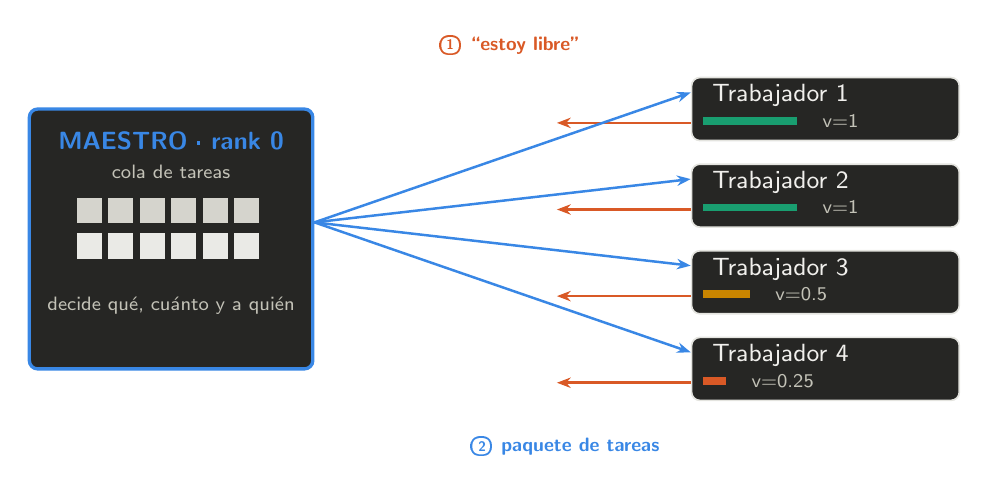
\begin{tikzpicture}
  % maestro
  \node[nodo,minimum width=3.6cm,minimum height=3.3cm,draw=azul,line width=1.2pt] (m) at (0,0) {};
  \node[font=\bfseries\small,text=azul] at (0,1.25) {MAESTRO · rank 0};
  \node[txtp] at (0,.85) {cola de tareas};
  \foreach \k in {0,...,5}{\fill[tinta2!70] ({-1.2+\k*.4},.2) rectangle ++(.32,.32);}
  \foreach \k in {0,...,5}{\fill[tinta2!35] ({-1.2+\k*.4},-.25) rectangle ++(.32,.32);}
  \node[txtp] at (0,-.85) {decide qué, cuánto y a quién};
  % trabajadores
  \foreach \i/\n/\v/\c in {0/{Trabajador 1}/1/aqua, 1/{Trabajador 2}/1/aqua, 2/{Trabajador 3}/0.5/ambar, 3/{Trabajador 4}/0.25/naranja}{
    \node[nodo,minimum width=3.4cm,minimum height=.8cm,anchor=west] (w\i) at (6.6,{1.65-\i*1.1}) {};
    \node[font=\small,text=tinta,anchor=west] at (6.75,{1.82-\i*1.1}) {\n};
    \fill[\c] (6.75,{1.45-\i*1.1}) rectangle ({6.75+1.2*\v},{1.45-\i*1.1+.1});
    \node[txtp,anchor=west] at ({6.95+1.2*\v},{1.5-\i*1.1}) {v=\v};
  }
  % mensajes
  \foreach \i in {0,...,3}{
    \draw[flecha,naranja] ([yshift=-5pt]w\i.west) -- ++(-1.7,0) coordinate (a\i);
    \draw[flecha,azul] ([yshift=6pt]m.east) -- ([yshift=6pt]w\i.west);
  }
  \node[font=\scriptsize\bfseries,text=naranja] at (4.3,2.45) {\textcircled{\tiny 1} “estoy libre”};
  \node[font=\scriptsize\bfseries,text=azul] at (5.0,-2.65) {\textcircled{\tiny 2} paquete de tareas};
\end{tikzpicture}
\fuente{El maestro solo coordina; el que se desocupa pide más trabajo (esquema bajo demanda; Fernandes et al., 2024).}
\note[item]{El maestro (rank 0) tiene la cola de tareas y no calcula. Los trabajadores son los nodos, cada uno con su velocidad.}
\note[item]{Dos mensajes: el trabajador dice ``estoy libre'' y el maestro responde con un paquete.}
\end{frame}

\begin{frame}{Protocolo de mensajes}
\centering
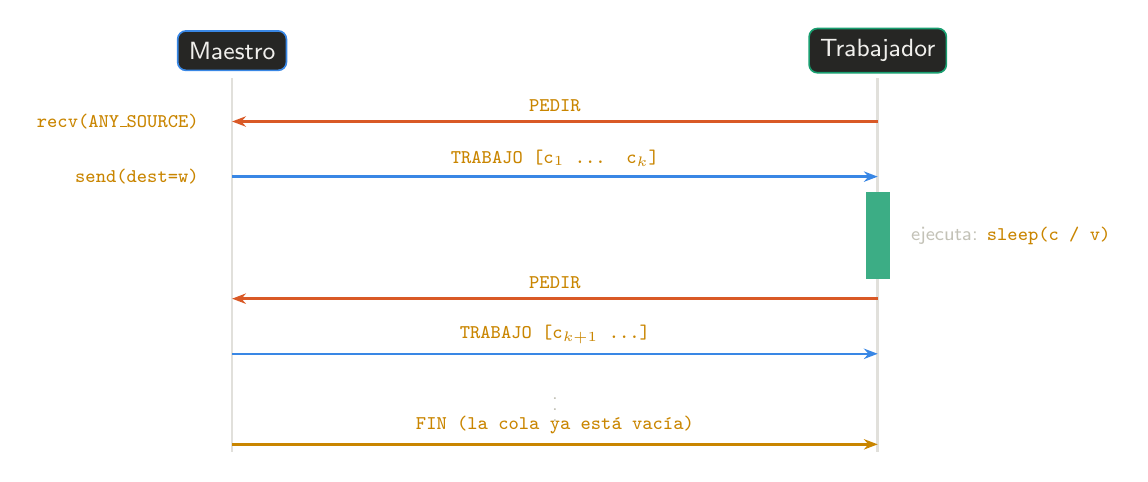
\begin{tikzpicture}[x=1cm,y=1cm]
  \node[nodo,draw=azul] (M) at (1.2,0) {Maestro};
  \node[nodo,draw=aqua] (T) at (9.4,0) {Trabajador};
  \draw[tinta2!50,line width=1pt] (1.2,-.35) -- (1.2,-5.1);
  \draw[tinta2!50,line width=1pt] (9.4,-.35) -- (9.4,-5.1);
  \draw[flecha,naranja] (9.4,-.9) -- (1.2,-.9) node[midway,above,txtm] {PEDIR};
  \draw[flecha,azul] (1.2,-1.6) -- (9.4,-1.6) node[midway,above,txtm] {TRABAJO [c$_1$ … c$_k$]};
  \fill[aqua!85] (9.25,-1.8) rectangle (9.55,-2.9);
  \node[txtp,anchor=west] at (9.7,-2.35) {ejecuta: \mono{sleep(c / v)}};
  \draw[flecha,naranja] (9.4,-3.15) -- (1.2,-3.15) node[midway,above,txtm] {PEDIR};
  \draw[flecha,azul] (1.2,-3.85) -- (9.4,-3.85) node[midway,above,txtm] {TRABAJO [c$_{k+1}$ …]};
  \node[txtp] at (5.3,-4.45) {$\vdots$};
  \draw[flecha,ambar] (1.2,-5.0) -- (9.4,-5.0) node[midway,above,txtm] {FIN  (la cola ya está vacía)};
  \node[txtm,anchor=east] at (.9,-.9) {recv(ANY\_SOURCE)};
  \node[txtm,anchor=east] at (.9,-1.6) {send(dest=w)};
\end{tikzpicture}
\note[item]{Tres tipos de mensaje: PEDIR, TRABAJO y FIN. En mpi4py el maestro usa recv con ANY\_SOURCE para atender al primero que pida.}
\note[item]{El trabajador es quien manda el ritmo: pide cuando termina. Eso es lo que hace al esquema dinámico.}
\end{frame}

\section{Estático vs. dinámico}
\begin{frame}{Estático vs.\ dinámico}
\begin{columns}[c,onlytextwidth]
\column{.6\textwidth}\centering
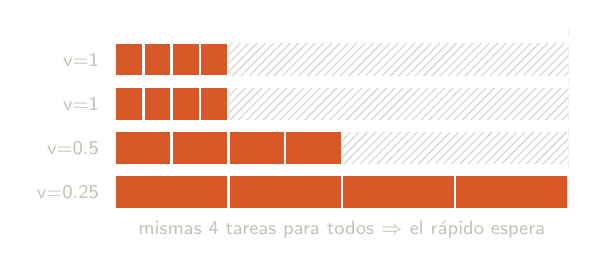
\begin{tikzpicture}[scale=.8]
  \foreach \i/\n/\w in {0/{v=1}/.45,1/{v=1}/.45,2/{v=0.5}/.9,3/{v=0.25}/1.8}{
    \node[txtp,anchor=east] at (-.1,{-\i*.7-.25}) {\n};
    \foreach \k in {1,...,4}{\fill[naranja] ({(\k-1)*\w+.02},{-\i*.7}) rectangle ({\k*\w-.02},{-\i*.7-.5});}
    \pgfmathsetmacro{\fin}{4*\w}
    \fill[pattern=north east lines,pattern color=tinta2!70] ({\fin},{-\i*.7}) rectangle (7.2,{-\i*.7-.5});
  }
  \draw[dashed,tinta] (7.2,.25) -- (7.2,-2.65);
  \node[txtp] at (3.6,-2.95) {mismas 4 tareas para todos $\Rightarrow$ el rápido espera};
\end{tikzpicture}
\column{.38\textwidth}
\begin{tarjeta}[height=2.45cm]{naranja}{Estático: se decide antes}
\small Reparto antes de ejecutar $\cdot$ 1 mensaje por nodo (\mono{Scatter}) $\cdot$ variantes: bloques, cíclico, ponderado
\end{tarjeta}
\end{columns}\vspace{5pt}
\begin{columns}[c,onlytextwidth]
\column{.6\textwidth}\centering
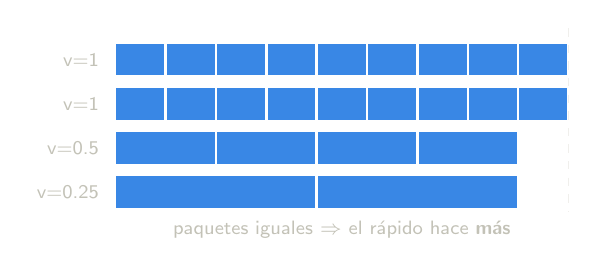
\begin{tikzpicture}[scale=.8]
  \foreach \i/\n/\w/\c in {0/{v=1}/.8/9,1/{v=1}/.8/9,2/{v=0.5}/1.6/4,3/{v=0.25}/3.2/2}{
    \node[txtp,anchor=east] at (-.1,{-\i*.7-.25}) {\n};
    \foreach \k in {1,...,9}{
      \ifnum\k>\c\relax\else
      \fill[azul] ({(\k-1)*\w+.02},{-\i*.7}) rectangle ({\k*\w-.02},{-\i*.7-.5});
      \fi}
  }
  \draw[dashed,tinta] (7.2,.25) -- (7.2,-2.65);
  \node[txtp] at (3.6,-2.95) {paquetes iguales $\Rightarrow$ el rápido hace \textbf{más}};
\end{tikzpicture}
\column{.38\textwidth}
\begin{tarjeta}[height=2.45cm]{azul}{Dinámico: pide el que se desocupa}
\small Cola en el maestro $\cdot$ no necesita conocer las velocidades $\cdot$ costo: $\approx 2$ mensajes por paquete
\end{tarjeta}
\end{columns}
\note[item]{Arriba, estático: el maestro decide todo al inicio. Con el mismo número de tareas para todos, el nodo rápido termina antes y espera (zona rayada).}
\note[item]{Abajo, dinámico: con paquetes iguales el nodo rápido pide más veces y hace más tareas; todos terminan casi juntos. El costo es la comunicación.}
\end{frame}

\begin{frame}[fragile]{Algoritmos: estático y dinámico}
\begin{columns}[T,onlytextwidth]
\column{.42\textwidth}
{\small\bfseries\color{naranja}Estático}
\begin{lstlisting}[style=ps]
// MAESTRO: decide TODO antes
PARA CADA nodo i EN 1..W:
    lote[i] <- tareas asignadas
          (bloque | cíclico | v_i)
SCATTER(lote)    // 1 msj por nodo

// TRABAJADOR i
lote <- RECIBIR
PARA CADA tarea EN lote:
    ejecutar(tarea)
BARRERA          // espera al más lento
\end{lstlisting}
\vspace{4pt}
\begin{tarjeta}[]{ambar}{Diferencia clave}
\small En el dinámico, \textbf{el ritmo lo marca el trabajador}.
\end{tarjeta}
\column{.56\textwidth}
{\small\bfseries\color{azul}Dinámico}
\begin{lstlisting}[style=ps]
// MAESTRO
cola <- todas las tareas
MIENTRAS haya nodos activos:
    i <- RECIBIR(cualquiera)
    SI cola no vacía ENTONCES
        ENVIAR(i, siguiente paquete)
    SINO
        ENVIAR(i, FIN)

// TRABAJADOR i
REPETIR
    ENVIAR(PEDIR)
    paquete <- RECIBIR
    SI paquete = FIN ENTONCES salir
    PARA CADA tarea EN paquete:
        ejecutar(tarea)
\end{lstlisting}
\end{columns}
\note[item]{Estático: el maestro arma los lotes, los envía con un Scatter y cada trabajador procesa lo suyo; la barrera final es la espera.}
\note[item]{Dinámico: el maestro atiende el primer PEDIR que llegue y responde con un paquete; termina cuando la cola se vacía y envía FIN. El código real está en el archivo aparte balanceo.py.}
\end{frame}

\begin{frame}{Cuadro comparativo: estático vs.\ dinámico}
\small\renewcommand{\arraystretch}{1.05}\arrayrulecolor{tinta2!35}
\begin{tabular}{@{}>{\bfseries\raggedright\arraybackslash}p{3.7cm}p{4.9cm}p{4.9cm}@{}}
\toprule
\color{tinta2}Criterio & \color{naranja}Estático & \color{azul}Dinámico \\ \midrule
Cuándo se reparte & Antes de ejecutar & Durante la ejecución \\
Mensajes & \ok{Pocos (1 por nodo)} & \ko{Muchos ($\approx 2$ por paquete)} \\
Nodos distintos o tareas desiguales & \ko{Espera el más rápido} & \ok{Se adapta solo} \\
Un nodo que se degrada & \ko{No reacciona} & \ok{Reparte menos a ese nodo} \\
Implementación & \ok{Simple} & Más compleja \\
Riesgo & Nodos en espera & Maestro como cuello de botella \\
\bottomrule
\end{tabular}
\fuente{Criterios basados en la descripción de la planificación static/dynamic/guided (OpenMP ARB, 2021) y en Pacheco \& Malensek (2022).}
\note[item]{Este es el cuadro resumen de la comparación. Subraya: estático gana en simplicidad y pocos mensajes; dinámico gana cuando hay heterogeneidad o cargas impredecibles.}
\end{frame}

\begin{frame}{¿Cómo se asignan los paquetes según la velocidad?}
\begin{columns}[c,onlytextwidth]
\column{.64\textwidth}
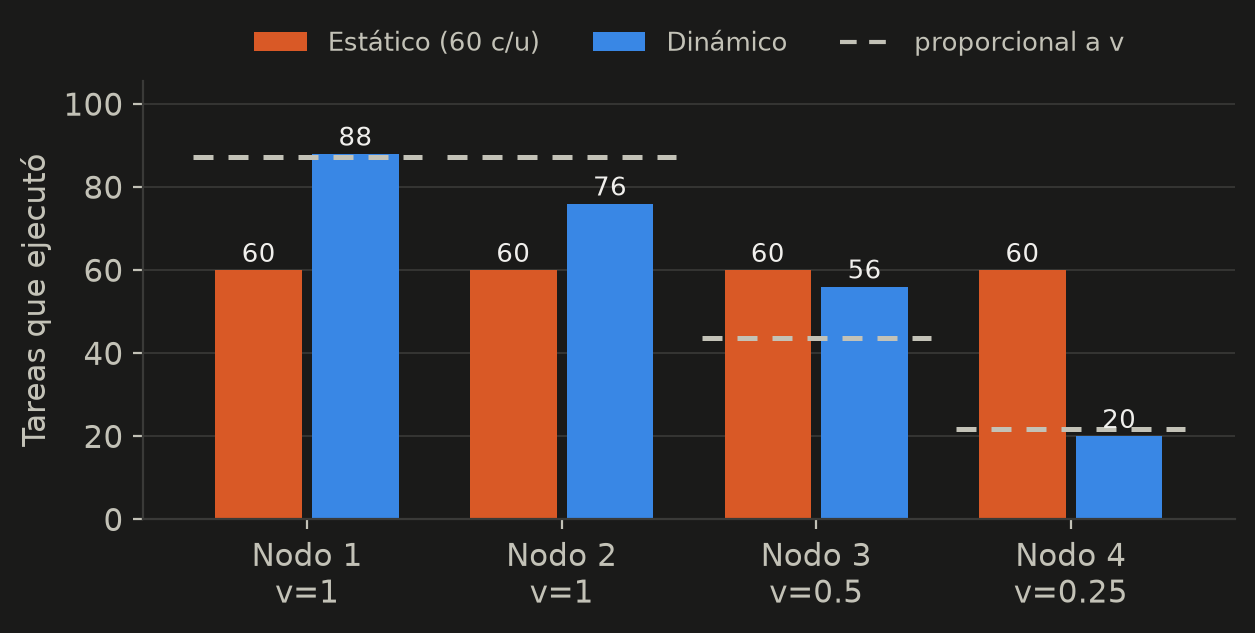
\includegraphics[width=\linewidth]{../resultados/figuras/tareas_nodo.png}
\column{.34\textwidth}
\begin{tarjeta}[]{azul}{Dinámico}
\small No se mide la velocidad: el nodo rápido \textbf{pide más veces}.
\end{tarjeta}\vspace{4pt}
\begin{tarjeta}[]{aqua}{Guiado}
\small $k=\max\!\big(k_{\min},\lceil \tfrac{\text{restantes}}{f\cdot W}\rceil\big)$\\
Paquetes \textbf{grandes al inicio}, chicos al final.
\end{tarjeta}
\end{columns}
\fuente{Equivale a las planificaciones dynamic y guided de OpenMP (OpenMP ARB, 2021).}
\note[item]{Respuesta a la pregunta del tema: el maestro nunca conoce las velocidades. El nodo rápido termina antes, pide antes y recibe más paquetes. Las líneas punteadas son el reparto ideal proporcional a la velocidad.}
\note[item]{Guiado: los primeros paquetes son grandes (menos mensajes) y se encogen al final para que nadie se quede con un paquete enorme cuando casi no hay trabajo.}
\end{frame}

\section{Evitar esperas}
\begin{frame}{Estrategias para evitar nodos en espera}
\begin{columns}[T,onlytextwidth]
\column{.32\textwidth}
\begin{tarjeta}[height=2.3cm]{aqua}{1 · Pedir bajo demanda}
\ok{\textbf{En el proyecto}.} Nadie espera si hay cola.
\end{tarjeta}\vspace{4pt}
\begin{tarjeta}[height=2.3cm]{ambar}{4 · Tareas pesadas primero}
Ordenar de mayor a menor costo (LPT).
\end{tarjeta}
\column{.32\textwidth}
\begin{tarjeta}[height=2.3cm]{aqua}{2 · Paquetes guiados}
\ok{\textbf{En el proyecto}.} Paquetes chicos al final.
\end{tarjeta}\vspace{4pt}
\begin{tarjeta}[height=2.3cm]{ambar}{5 · Prefetch}
Pedir el siguiente paquete \textbf{antes} de terminar.
\end{tarjeta}
\column{.32\textwidth}
\begin{tarjeta}[height=2.3cm]{aqua}{3 · Ponderar por velocidad}
\ok{\textbf{En el proyecto}.} Si $v_i$ es conocida y estable.
\end{tarjeta}\vspace{4pt}
\begin{tarjeta}[height=2.3cm]{ambar}{6 · Robo de trabajo}
El ocioso \textbf{roba} tareas a otro (sin maestro).
\end{tarjeta}
\end{columns}
\fuente{Robo de trabajo adaptativo en sistemas heterogéneos: Fernandes et al. (2024).}
\note[item]{Las tres primeras las implementé y las medí. Las otras tres son estrategias de la literatura que quedan como trabajo futuro.}
\note[item]{Prefetch y robo de trabajo se explican en la siguiente diapositiva y en las conclusiones.}
\end{frame}

\section{Simulación}
\begin{frame}{Simulación en una laptop y diseño experimental}
\begin{columns}[T,onlytextwidth]
\column{.5\textwidth}\centering
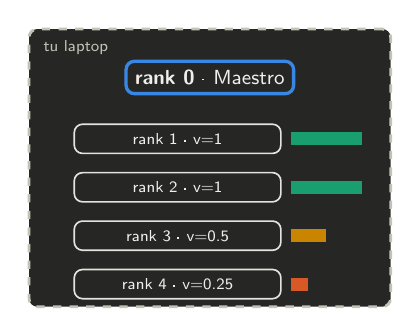
\begin{tikzpicture}[scale=.82,transform shape]
  \node[nodo,minimum width=5.6cm,minimum height=4.3cm,draw=tinta2,dashed,line width=1pt] at (0,0) {};
  \node[txtp,anchor=north west] at (-2.7,2.1) {tu laptop};
  \node[nodo,draw=azul,line width=1.2pt] at (0,1.4) {\textbf{rank 0} · Maestro};
  \foreach \i/\v/\c/\t in {0/1.0/aqua/{rank 1 · v=1}, 1/1.0/aqua/{rank 2 · v=1}, 2/0.5/ambar/{rank 3 · v=0.5}, 3/0.25/naranja/{rank 4 · v=0.25}}{
    \node[nodo,minimum width=3.2cm] at (-.5,{.45-\i*.75}) {\scriptsize \t};
    \fill[\c] (1.25,{.45-\i*.75-.1}) rectangle ++({1.1*\v},.2);
  }
\end{tikzpicture}
\column{.47\textwidth}
\footnotesize\renewcommand{\arraystretch}{1.1}
\begin{tabular}{@{}p{3cm}p{2.7cm}@{}}
\toprule
\color{azul}Real & \color{aqua}Simulado \\ \midrule
Nodo & proceso MPI \\
Velocidad & factor $v$ \\
Cómputo & \mono{sleep(c/v)} \\
Red lenta & \mono{--latencia-ms} \\
Nodo que se degrada & \mono{--degradar} \\ \bottomrule
\end{tabular}
\end{columns}\vspace{4pt}
\begin{tarjeta}[]{ambar}{Escenarios medidos}
\scriptsize Nodos iguales $\cdot$ nodos distintos ($v=1,1,0.5,0.25$) $\cdot$ tamaño de paquete (1…60, latencia 3\,ms) $\cdot$ 1, 2, 4 y 8 trabajadores $\cdot$ un nodo que se degrada.\\
240 tareas $\cdot$ costo medio 10\,ms (log-normal) $\cdot$ semilla fija $\cdot$ mediana de 3--5 corridas $\cdot$ código en \mono{balanceo.py} (archivo aparte).
\end{tarjeta}
\note[item]{En una laptop todos los procesos son igual de rápidos, entonces simulo la heterogeneidad: cada trabajador tiene un factor de velocidad y tarda costo dividido entre velocidad. Con mpiexec -n 5 hay 1 maestro y 4 trabajadores.}
\note[item]{Usar sleep hace que los resultados no dependan de cuántos núcleos tenga la laptop. También existe un modo real con carga de CPU.}
\note[item]{Cinco escenarios, cada uno con una pregunta: ¿qué pasa con nodos iguales?, ¿con nodos distintos?, ¿cuál es el mejor tamaño de paquete?, ¿cómo escala?, ¿qué pasa si un nodo se degrada? Mismas tareas (semilla fija) para todas las estrategias.}
\end{frame}

\section{Resultados}
\begin{frame}{Línea de tiempo: quién trabaja y quién espera}
\centering
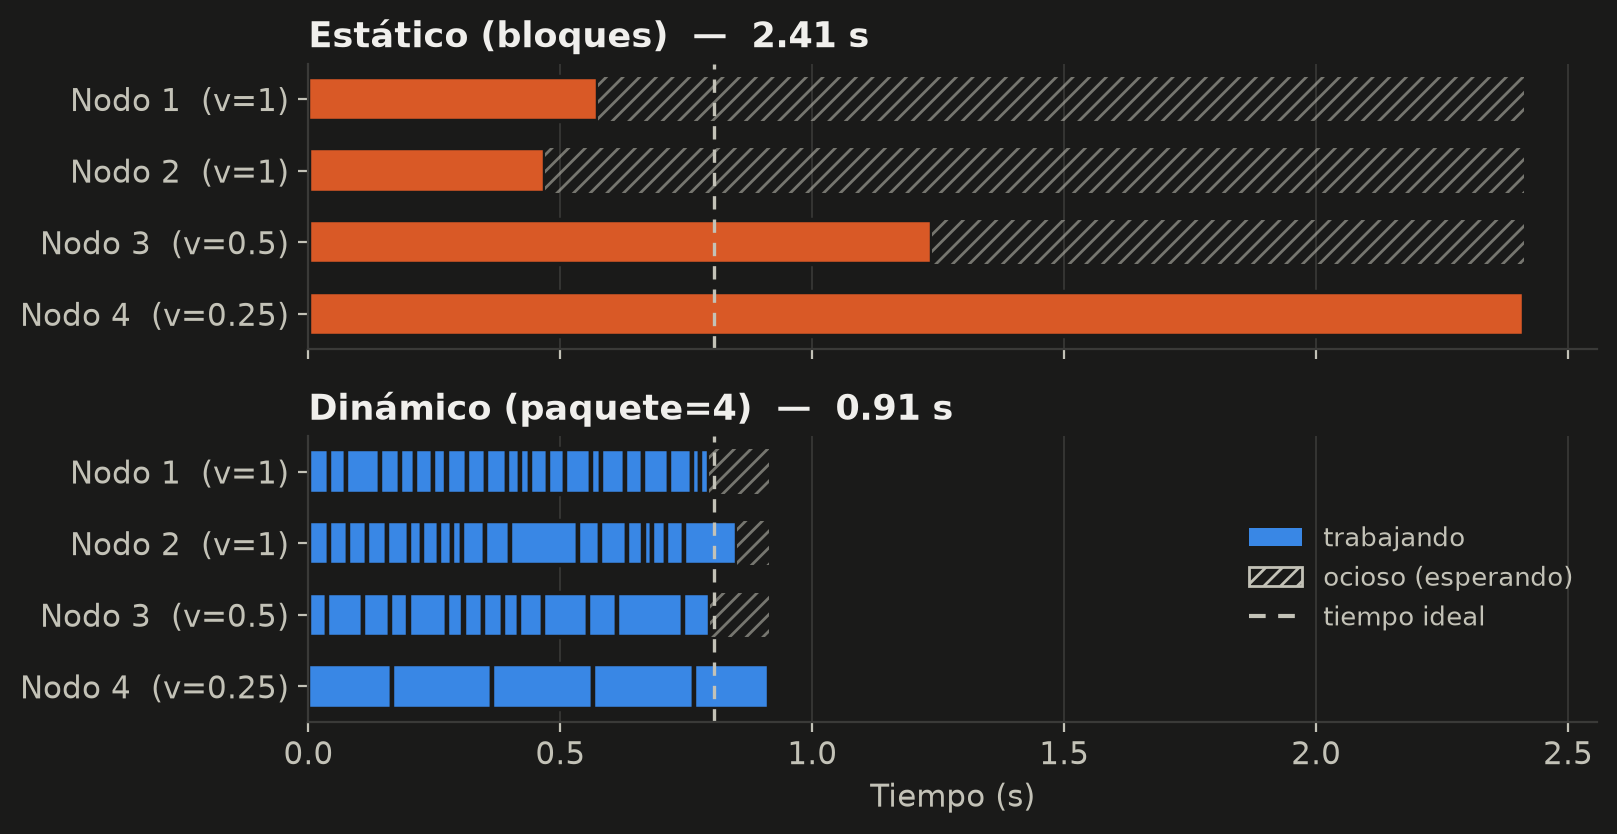
\includegraphics[width=\linewidth,height=5.3cm,keepaspectratio]{../resultados/figuras/gantt.png}\\[3pt]
{\large Utilización media: estático \ko{\utEstHet\,\%} $\;\rightarrow\;$ dinámico \ok{\utDinHet\,\%}}
\note[item]{Esta es la diapositiva más importante. Naranja arriba: el nodo 4 trabaja todo el tiempo y los demás están hachurados, es decir, esperando.}
\note[item]{Abajo, con dinámico, todos terminan casi al mismo tiempo, cerca de la línea punteada de tiempo ideal.}
\end{frame}

\begin{frame}{Tiempo total: nodos distintos y nodo degradado}
\centering
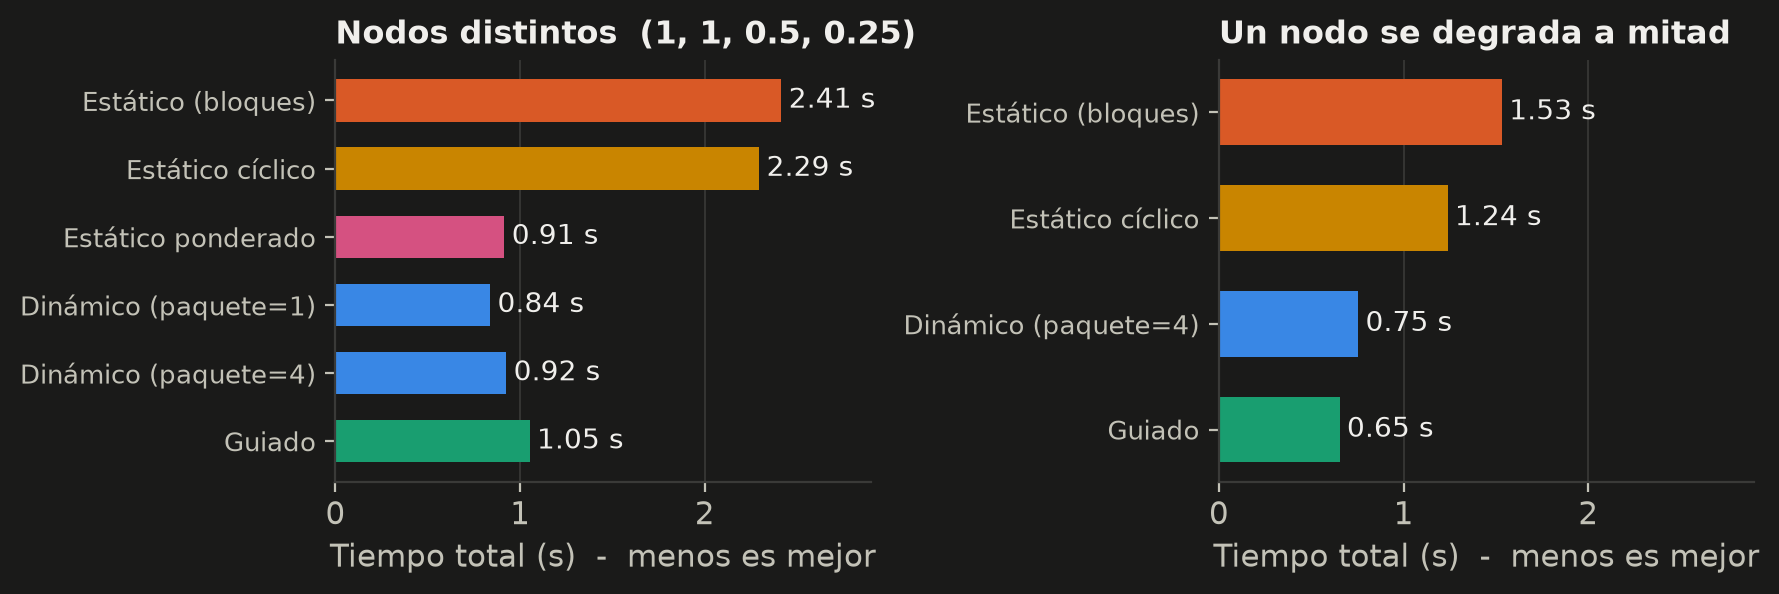
\includegraphics[width=\linewidth,height=4.9cm,keepaspectratio]{../resultados/figuras/tiempos.png}\\[4pt]
{\large Nodos distintos: dinámico \textbf{\mejoraHet$\times$} más rápido $\;\bullet\;$ nodo degradado: \textbf{\mejoraDeg$\times$}}\\[2pt]
{\small\color{tinta2}Con nodos iguales casi empatan: \tEstHom\,s (estático) vs.\ \tDinHom\,s (dinámico).}
\note[item]{Con nodos iguales estático y dinámico casi empatan: no hay nada que balancear. Con nodos distintos, el estático tarda \tEstHet{} s y el dinámico \tDinHet{} s.}
\note[item]{A la derecha el caso más duro: un nodo baja de velocidad a mitad de la ejecución y nadie lo sabía de antemano. Ahí ni siquiera el estático ponderado ayudaría; solo el dinámico reacciona.}
\end{frame}

\begin{frame}{Tamaño del paquete}
\centering
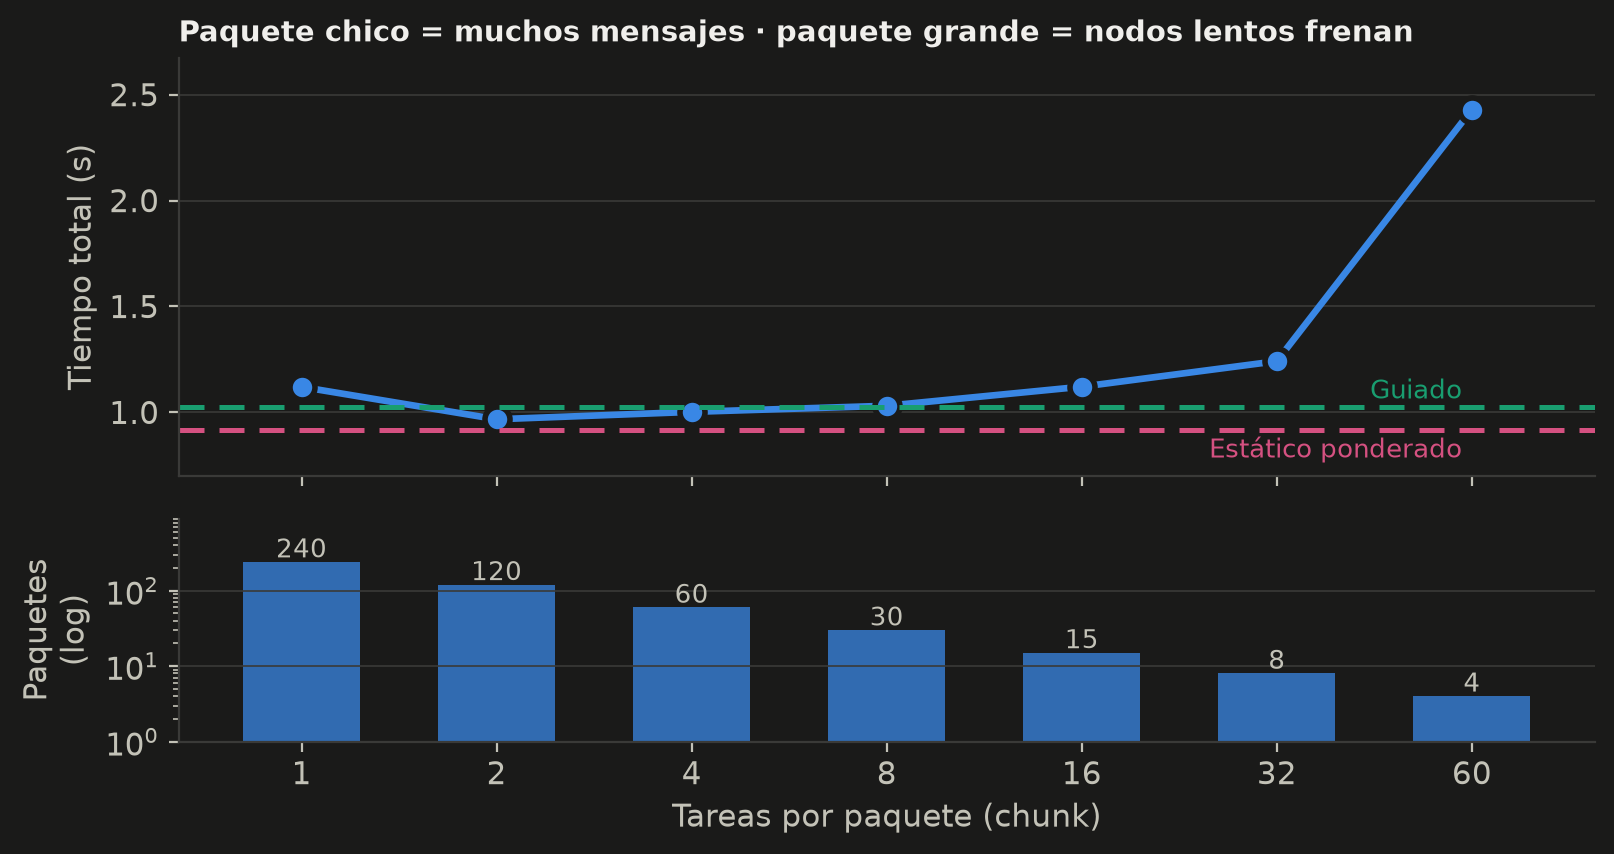
\includegraphics[width=\linewidth,height=6.2cm,keepaspectratio]{../resultados/figuras/chunk.png}
\note[item]{Hay un compromiso: paquetes muy chicos generan muchos mensajes; paquetes muy grandes dejan a un nodo lento con demasiado trabajo.}
\note[item]{Con paquete de 60 tareas, un solo nodo lento recibe un paquete enorme y el tiempo se dispara a más de 2 segundos, igual de malo que el estático.}
\end{frame}

\begin{frame}{Escalabilidad: más nodos}
\centering
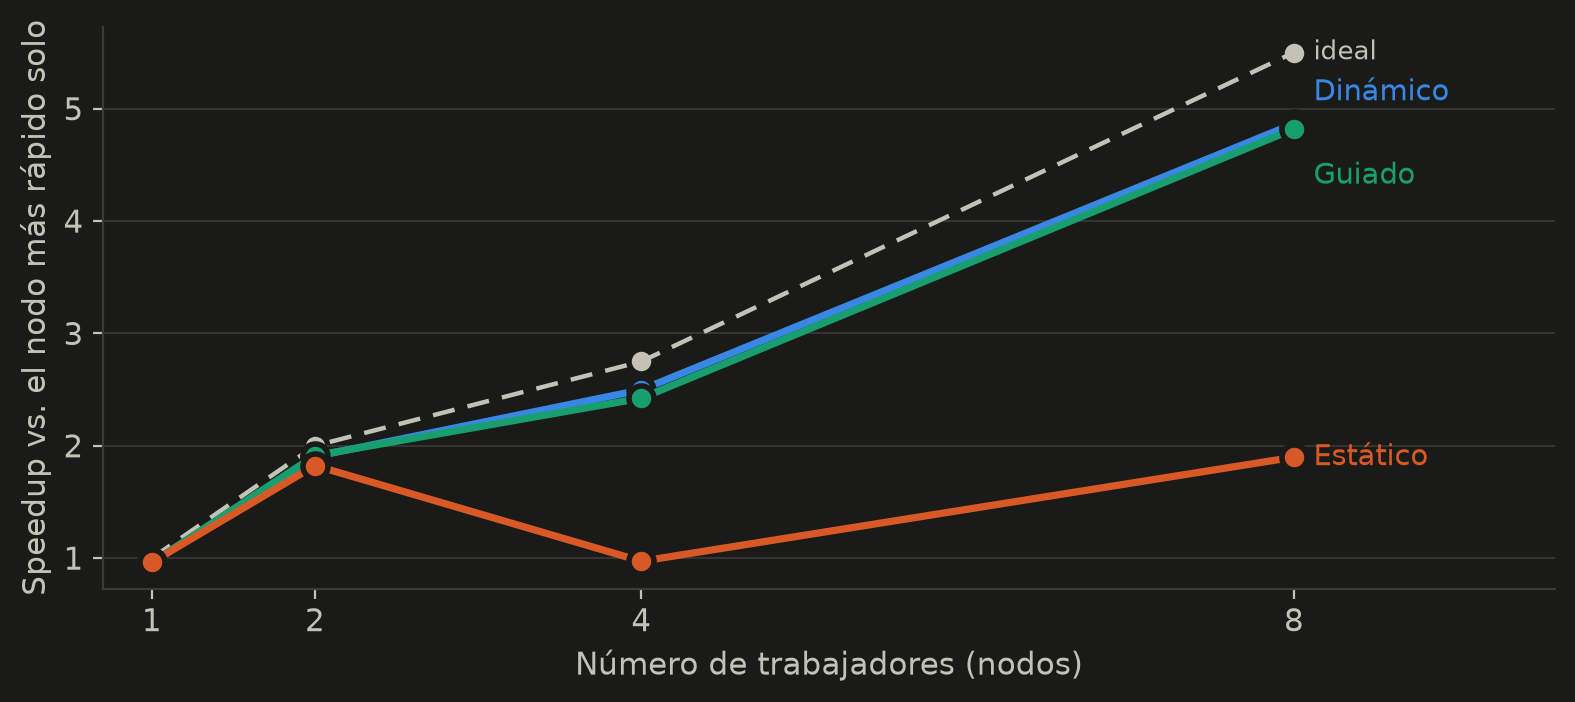
\includegraphics[width=\linewidth,height=6.2cm,keepaspectratio]{../resultados/figuras/escalabilidad.png}
\note[item]{Speedup contra un nodo rápido trabajando solo. El estático casi no mejora porque lo frena el nodo más lento; el dinámico se acerca al ideal.}
\note[item]{Con 8 trabajadores el dinámico logra \spDinOcho$\times$ y el estático solo \spEstOcho$\times$.}
\end{frame}

\section{Cierre}
\begin{frame}{Conclusiones y trabajo futuro}
\begin{columns}[T,onlytextwidth]
\column{.56\textwidth}
\begin{tarjeta}[height=1.5cm]{azul}{1 · Estático}
\small Simple y barato, pero un nodo lento frena a todos (\tEstHet\,s).
\end{tarjeta}\vspace{4pt}
\begin{tarjeta}[height=1.5cm]{aqua}{2 · Dinámico}
\small Asigna paquetes a quien se desocupa, sin conocer velocidades (\tDinHet\,s).
\end{tarjeta}\vspace{4pt}
\begin{tarjeta}[height=1.5cm]{naranja}{3 · El paquete importa}
\small Ni muy chico ni muy grande; el guiado no siempre gana (\tGuiHet\,s).
\end{tarjeta}
\column{.42\textwidth}
\begin{tarjeta}[height=2.35cm]{ambar}{Limitaciones}
\begin{itemize}\setlength\itemsep{1pt}\footnotesize
\item Nodos simulados (\mono{sleep}), sin red física
\item Una sola laptop
\item El maestro puede ser cuello de botella
\end{itemize}
\end{tarjeta}\vspace{4pt}
\begin{tarjeta}[height=2.35cm]{aqua}{Trabajo futuro}
\begin{itemize}\setlength\itemsep{1pt}\footnotesize
\item Prefetch con \mono{isend/irecv}
\item Robo de trabajo sin maestro
\item Probar en un cluster real
\end{itemize}
\end{tarjeta}
\end{columns}
\note[item]{Tres ideas para cerrar: estático simple pero frágil; dinámico se adapta; y el tamaño del paquete es la perilla importante (el guiado no siempre gana porque su primer paquete grande puede caer en el nodo lento).}
\note[item]{Regla práctica: si no conozco las velocidades o no son estables, dinámico. Si las conozco y las tareas son parejas, estático ponderado es más simple y barato.}
\note[item]{Sé honesto con las limitaciones: la simulación es una abstracción; en un cluster real habría red, memoria y contención.}
\end{frame}

\begin{frame}{¿Preguntas? · Referencias}
\begin{columns}[T,onlytextwidth]
\column{.28\textwidth}
{\fontsize{19}{21}\selectfont\bfseries\color{tinta}¿Preguntas?}\\[6pt]
{\small\color{tinta2}Gracias por su atención}\\[10pt]
{\scriptsize\ttfamily\color{ambar}\integrantes}
\column{.68\textwidth}
\fontsize{7.2}{9}\selectfont\setlength{\parindent}{-1.2em}\leftskip1.2em\raggedright
Dalcin, L., \& Fang, Y.-L. L. (2021). mpi4py: Status update after 12 years of development. \emph{Computing in Science \& Engineering, 23}(4), 47–54. \url{https://doi.org/10.1109/MCSE.2021.3083216}\par\vspace{3pt}
Fernandes, J. B., de Assis, Í. A. S., Martins, I. M. S., Barros, T., \& Xavier-de-Souza, S. (2024). \emph{Adaptive asynchronous work-stealing for distributed load-balancing in heterogeneous systems} [Preprint]. arXiv. \url{https://arxiv.org/abs/2401.04494}\par\vspace{3pt}
Message Passing Interface Forum. (2023). \emph{MPI: A message-passing interface standard, version 4.1}. \url{https://www.mpi-forum.org/docs/mpi-4.1/mpi41-report/mpi41-report.htm}\par\vspace{3pt}
OpenMP Architecture Review Board. (2021). \emph{OpenMP application programming interface, version 5.2}. \url{https://www.openmp.org/specifications/}\par\vspace{3pt}
Pacheco, P. S., \& Malensek, M. (2022). \emph{An introduction to parallel programming} (2nd ed.). Morgan Kaufmann.\par\vspace{3pt}
Rogowski, M., Aseeri, S., Keyes, D., \& Dalcin, L. (2023). mpi4py.futures: MPI-based asynchronous task execution for Python. \emph{IEEE Transactions on Parallel and Distributed Systems, 34}(2), 611–622.
\end{columns}
\note[item]{Todas las referencias son de 2021 en adelante, en formato APA 7.}
\note[item]{Preguntas frecuentes: ¿por qué sleep? (reproducible y sin depender de núcleos); ¿por qué el guiado fue peor? (primer paquete grande en el nodo lento); ¿qué pasa si el maestro falla? (trabajo futuro).}
\end{frame}

\end{document}
